\documentclass[aspectratio=169,11pt]{beamer}

\usepackage{fontspec}
\usepackage{amsmath,amssymb,bm,mathtools}
\usepackage{booktabs,tabularx,array}
\usepackage{graphicx}
\usepackage{tikz}
\usetikzlibrary{arrows.meta,positioning,shapes.geometric,calc}

\setmainfont{TeX Gyre Pagella}
\setsansfont{TeX Gyre Heros}
\setmonofont{Latin Modern Mono}
\usefonttheme{professionalfonts}

\definecolor{navy}{HTML}{183A5A}
\definecolor{teal}{HTML}{087E8B}
\definecolor{orange}{HTML}{E07A3F}
\definecolor{green}{HTML}{3E8E63}
\definecolor{red}{HTML}{B94A48}
\definecolor{ink}{HTML}{27323A}
\definecolor{muted}{HTML}{65727C}

\setbeamercolor{normal text}{fg=ink,bg=white}
\setbeamercolor{structure}{fg=teal}
\setbeamercolor{frametitle}{fg=navy,bg=white}
\setbeamercolor{title}{fg=navy}
\setbeamercolor{subtitle}{fg=muted}
\setbeamercolor{block title}{fg=white,bg=teal}
\setbeamercolor{block body}{fg=ink,bg=teal!6}
\setbeamercolor{alerted text}{fg=orange}
\setbeamercolor{itemize item}{fg=teal}
\setbeamercolor{itemize subitem}{fg=orange}

\setbeamertemplate{navigation symbols}{}
\setbeamertemplate{itemize item}{\raise0.15ex\hbox{\scriptsize$\blacktriangleright$}}
\setbeamertemplate{itemize subitem}{\raise0.15ex\hbox{\tiny$\blacktriangleright$}}
\setbeamertemplate{frametitle}{%
  \vspace{0.3em}\insertframetitle\par
  \vspace{-0.35em}{\color{teal}\rule{\textwidth}{0.7pt}}
}
\setbeamertemplate{footline}{%
  \leavevmode
  \hbox{%
    \begin{beamercolorbox}[wd=.78\paperwidth,ht=2.7ex,dp=1.1ex,leftskip=1em]{author in head/foot}%
      \color{muted}\scriptsize Reducing Hartree cost in KS--SCF
    \end{beamercolorbox}%
    \begin{beamercolorbox}[wd=.22\paperwidth,ht=2.7ex,dp=1.1ex,rightskip=1em plus1fil]{date in head/foot}%
      \color{muted}\scriptsize \insertframenumber/\inserttotalframenumber
    \end{beamercolorbox}%
  }
}

\newcommand{\norm}[1]{\left\lVert #1\right\rVert}
\newcommand{\mesh}{\mathcal T}

\title{Reducing Hartree Cost during Kohn--Sham SCF}
\subtitle{Mesh-update strategies, structure reuse, and method-selection experiments}
\author{Research progress and open discussion}
\date{September 2026}

\begin{document}

% 1
\begin{frame}[plain]
  \vspace{0.35cm}
  {\color{teal}\rule{\textwidth}{1.3pt}}
  \vspace{0.4cm}

  {\fontsize{25}{31}\selectfont\bfseries\sffamily\color{navy}
   Reducing Hartree Cost\par
   \vspace{0.15cm}during Kohn--Sham SCF\par}

  \vspace{0.4cm}
  {\Large\sffamily\color{muted}
   Mesh-update strategies, structure reuse, and comparison experiments}

  \vspace{0.5cm}
  \begin{beamercolorbox}[rounded=true,sep=0.55em,wd=0.92\textwidth]{block body}
    \centering
    \textbf{Open question:} which update strategy saves the most time
    \alert{without degrading SCF accuracy, convergence, or robustness?}
  \end{beamercolorbox}

  \vfill
  \hfill{\color{muted}\sffamily Group meeting \quad September 2026}
\end{frame}

% 2
\begin{frame}{Former work: one-step adaptive Hartree evaluation}
  \begin{columns}[T,onlytextwidth]
    \column{0.48\textwidth}
      \centering
      \small
      \[
        V_H(\bm x)=\int_\Omega
        \frac{\rho(\bm y)}{|\bm x-\bm y|}\,\mathrm d\bm y.
      \]
      \vspace{-0.18cm}
      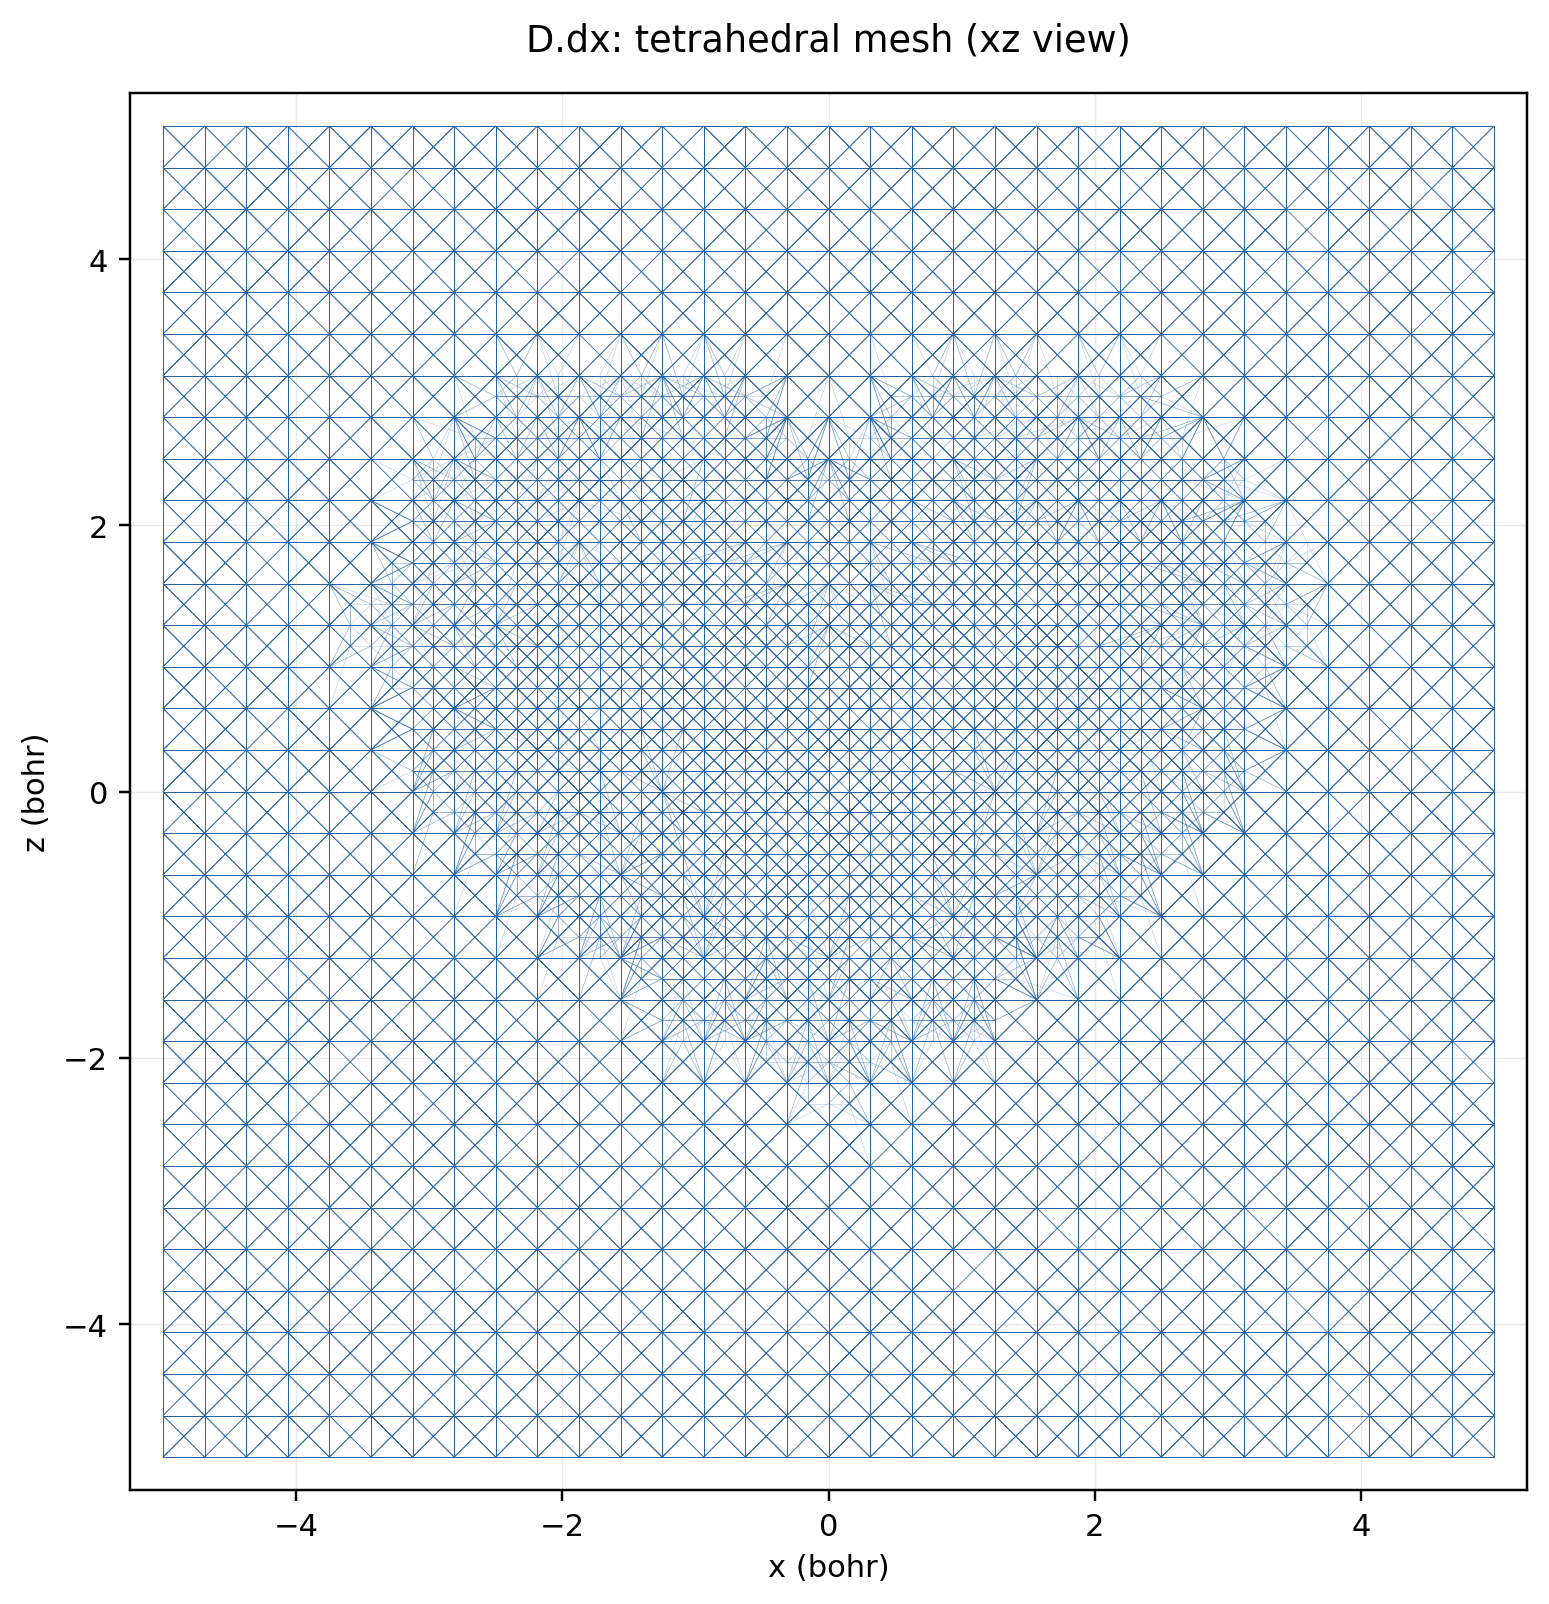
\includegraphics[
        height=4.55cm,
        trim=45 50 45 55,
        clip
      ]{D_mesh_fine.png}

      \vspace{-0.06cm}
      {\scriptsize\color{muted}
      Adaptive tetrahedral mesh: fine near the active source region and
      coarse in the far field.}
    \column{0.49\textwidth}
      \begin{block}{Matched CPU/GPU run}
        \centering
        {\scriptsize $n=120\,816$, $p=6$, $P=4$, $\theta=0.5$}

        \vspace{0.10cm}
        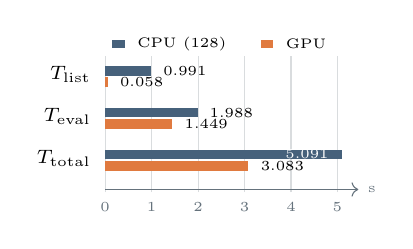
\begin{tikzpicture}[x=0.59cm,y=0.59cm]
          \foreach \x in {0,1,...,5}{
            \draw[muted!25] (\x,0.12)--(\x,3.05);
            \node[below,font=\tiny\color{muted}] at (\x,0.10) {\x};
          }
          \draw[->,draw=muted] (0,0.18)--(5.45,0.18)
            node[right,font=\tiny\color{muted}] {s};

          \node[anchor=east,font=\scriptsize] at (-0.10,2.65) {$T_{\rm list}$};
          \fill[navy!80] (0,2.63) rectangle (0.991,2.84);
          \fill[orange]  (0,2.38) rectangle (0.058,2.59);
          \node[anchor=west,font=\tiny] at (1.04,2.735) {0.991};
          \node[anchor=west,font=\tiny] at (0.11,2.485) {0.058};

          \node[anchor=east,font=\scriptsize] at (-0.10,1.75) {$T_{\rm eval}$};
          \fill[navy!80] (0,1.73) rectangle (1.988,1.94);
          \fill[orange]  (0,1.48) rectangle (1.449,1.69);
          \node[anchor=west,font=\tiny] at (2.04,1.835) {1.988};
          \node[anchor=west,font=\tiny] at (1.50,1.585) {1.449};

          \node[anchor=east,font=\scriptsize] at (-0.10,0.85) {$T_{\rm total}$};
          \fill[navy!80] (0,0.83) rectangle (5.091,1.04);
          \fill[orange]  (0,0.58) rectangle (3.083,0.79);
          \node[anchor=east,font=\tiny\color{white}] at (5.02,0.935) {5.091};
          \node[anchor=west,font=\tiny] at (3.14,0.685) {3.083};

          \fill[navy!80] (0.15,3.23) rectangle (0.42,3.40);
          \node[anchor=west,font=\tiny] at (0.48,3.315) {CPU (128)};
          \fill[orange] (3.35,3.23) rectangle (3.62,3.40);
          \node[anchor=west,font=\tiny] at (3.68,3.315) {GPU};
        \end{tikzpicture}

        \vspace{-0.02cm}
        {\scriptsize
        Same $L^2$ error: $2.2605\times10^{-4}$\par
        \alert{\(1.65\times\) end-to-end speedup}}
      \end{block}
      \vspace{0.04cm}
      {\tiny
      \textcolor{teal}{\textbf{List:}} independent target traversals and flat
      CSR storage give a large kernel gain.\par
      \textcolor{teal}{\textbf{Evaluation:}} irregular near-field quadrature
      and memory access limit the gain.\par
      \textcolor{teal}{\textbf{Total:}} host preparation and transfers reduce
      the end-to-end speedup.\par
      \color{muted}$T_{\rm list}$ is a backend timer; use $T_{\rm total}$ for
      the primary comparison.}
  \end{columns}
\end{frame}

% 3
\begin{frame}{KS--SCF turns one Hartree solve into repeated work}
  \small
  \[
    \left[-\frac12\Delta+V_{\mathrm{ext}}+V_H[\rho]+V_{\mathrm{xc}}[\rho]\right]
    \psi_i=\varepsilon_i\psi_i,
    \qquad
    \rho=\sum_i f_i|\psi_i|^2.
  \]

  \centering
  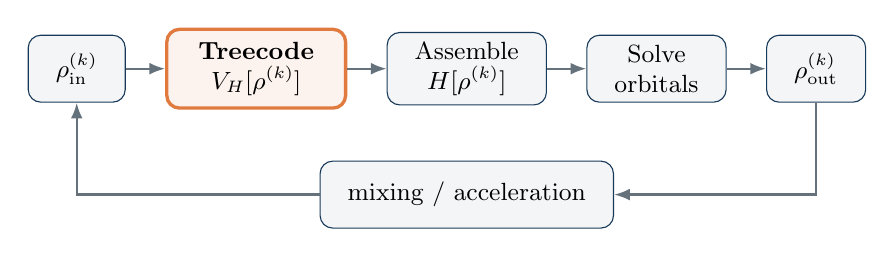
\begin{tikzpicture}[
      node distance=5mm,
      box/.style={draw=navy,rounded corners=1.6mm,fill=navy!5,
        minimum height=8.5mm,align=center,font=\small,inner xsep=3.5mm},
      hbox/.style={draw=orange,very thick,rounded corners=1.6mm,fill=orange!9,
        minimum height=10mm,align=center,font=\small\bfseries,inner xsep=4mm},
      arr/.style={-{Latex[length=2mm]},thick,draw=muted}]
    \node[box] (rho) {$\rho_{\rm in}^{(k)}$};
    \node[hbox,right=of rho] (hartree) {Treecode\\$V_H[\rho^{(k)}]$};
    \node[box,right=of hartree] (ham) {Assemble\\$H[\rho^{(k)}]$};
    \node[box,right=of ham] (eig) {Solve\\orbitals};
    \node[box,right=of eig] (out) {$\rho_{\rm out}^{(k)}$};
    \node[box,below=7mm of ham] (mix) {mixing / acceleration};
    \draw[arr] (rho)--(hartree);
    \draw[arr] (hartree)--(ham);
    \draw[arr] (ham)--(eig);
    \draw[arr] (eig)--(out);
    \draw[arr] (out.south) |- (mix.east);
    \draw[arr] (mix.west) -| (rho.south);
  \end{tikzpicture}

  \vspace{0.25cm}
  \begin{beamercolorbox}[rounded=true,sep=0.38em,wd=0.95\textwidth]{block body}
    \centering
    \(
      T_H^{(k)}=T_{\mathrm{density}}+T_{\mathrm{moment}}+T_{\mathrm{eval}}
      +I_k\bigl(T_{\mathrm{mesh}}+T_{\mathrm{tree/list}}+T_{\mathrm{transfer}}\bigr).
    \)
    \par\smallskip
    Every method recomputes the density-dependent terms. The open choice is when and
    how to update the mesh-dependent terms ($I_k=0$ or $1$).
  \end{beamercolorbox}
\end{frame}

% 4
\begin{frame}{What can be reused, and what remains density-dependent?}
  \begin{columns}[T,onlytextwidth]
    \column{0.49\textwidth}
      \begin{block}{Mesh-dependent data: potentially reusable}
        \small
        \begin{itemize}\setlength\itemsep{0.38em}
          \item tetrahedra, Jacobians, and quadrature locations;
          \item hierarchy and parent--child relations;
          \item neighbor/non-neighbor MAC lists;
          \item singular-integration geometry;
          \item GPU CSR indices and static allocations.
        \end{itemize}
      \end{block}
    \column{0.49\textwidth}
      \begin{block}{Density-dependent data: recompute each step}
        \small
        \begin{itemize}\setlength\itemsep{0.48em}
          \item density and source charge at quadrature points;
          \item leaf and aggregated multipole moments;
          \item direct neighbor contribution;
          \item non-neighbor multipole contribution;
          \item current Hartree potential and energy.
        \end{itemize}
      \end{block}
  \end{columns}

  \vspace{0.25cm}
  \centering\alert{We reuse the computational structure, not the previous Hartree potential.}
\end{frame}

% 5
\begin{frame}{Related methods and application settings}
  \centering
  \scriptsize
  \renewcommand{\arraystretch}{1.18}
  \setlength{\tabcolsep}{4pt}
  \begin{tabularx}{0.98\textwidth}{
      >{\raggedright\arraybackslash}p{2.75cm}
      >{\raggedright\arraybackslash}p{3.65cm}
      >{\raggedright\arraybackslash}X}
    \toprule
    Study & Application environment & Relevant mechanism\\
    \midrule
    Bao--Hu--Liu (2013)
      & Ground-state KS--DFT; moving finite-element mesh
      & Converge SCF on the current mesh, then redistribute the mesh.\\
    Bao--Hu--Liu (2015)
      & Real-time TDDFT; adaptive finite elements
      & Spatial and temporal residuals identify local trouble regions.\\
    Chen et al. (2014)
      & Ground-state KS--DFT; adaptive finite elements
      & Residual estimator and Dörfler marking select local refinement.\\
    Kuang--Shen--Hu (2024)
      & All-electron KS--DFT; multi-mesh finite elements
      & Separate orbital and Hartree meshes avoid a globally over-refined union mesh.\\
    Cui--Yang (2025)
      & Poisson treecode on general domains
      & Interaction-wise expansion order and direct/multipole switching.\\
    Keller et al. (2023), Cornerstone
      & GPU N-body and SPH particle simulations
      & SFC reordering, linear octrees, and device-resident tree construction.\\
    \bottomrule
  \end{tabularx}

  \vspace{0.22cm}
  \begin{beamercolorbox}[rounded=true,sep=0.3em,wd=0.94\textwidth]{block body}
    \centering\footnotesize
    These methods address different models; they provide design references,
    not a ranking for our implementation.
  \end{beamercolorbox}
\end{frame}

% 6
\begin{frame}{Controlled 20-step mesh-policy experiment}
  \begin{columns}[T,onlytextwidth]
    \column{0.57\textwidth}
      \footnotesize
      On $\Omega=[-5,5]^3$ and for artificial steps $k=0,\ldots,19$:
      \[
        V_k(\bm x)=
        \underbrace{V_0(\bm x)}_{\color{navy}\text{stationary}}
        +\underbrace{\beta_k}_{\color{orange}\text{amplitude}}\,
        \underbrace{V_1(\bm x-\bm c_k)}_{\color{teal}\text{moving Gaussian}} .
      \]
      \vspace{-0.08cm}
      \scriptsize
      \renewcommand{\arraystretch}{1.13}
      \begin{tabularx}{0.98\linewidth}{
          @{}>{\color{teal}\bfseries}p{0.82cm}X@{}}
        \(V_0\) & stationary Gaussian
          \(e^{-\pi(4x^2+8y^2+12z^2)}\)\\
        \(V_1\) & moving profile
          \(e^{-\pi(6\xi_x^2+5\xi_y^2+9\xi_z^2)}\)\\
        \(\beta_k\) & perturbation amplitude
          \(0.5(0.95)^k\); not SCF mixing\\
        \(\bm c_k\) & center
          \(\bigl(0.70+0.80(0.95)^k,-0.35,0.20\bigr)\)\\
        \(\rho_k\) & analytic source
          \(-(4\pi)^{-1}\Delta V_k\); hence \(V_k\) is exact\\
      \end{tabularx}

      \vspace{0.08cm}
      {\scriptsize\color{muted}
      CPU backend; 128 OpenMP threads; $p=6$, $P=4$, $\theta=0.5$;
      adaptive tolerance $10^{-6}$.}
    \column{0.40\textwidth}
      \begin{block}{Six implemented policies}
        \footnotesize
        \begin{itemize}\setlength\itemsep{0.24em}
          \item \texttt{FROZEN};
          \item \texttt{EVERY\_H};
          \item \texttt{PERIODIC\_H};
          \item \texttt{RESIDUAL\_H};
          \item \texttt{MOVING\_R};
          \item \texttt{HYBRID\_HR}.
        \end{itemize}
      \end{block}
      \vspace{-0.18cm}
      \begin{block}{Recorded quantities}
        \scriptsize
        element count, update type, list/moment/evaluation time,
        sequence time, $L^2$ error, displacement, and mesh quality.
      \end{block}
  \end{columns}
\end{frame}

% 7
\begin{frame}{Main result: residual-controlled $h$-updates lead this test}
  \centering
  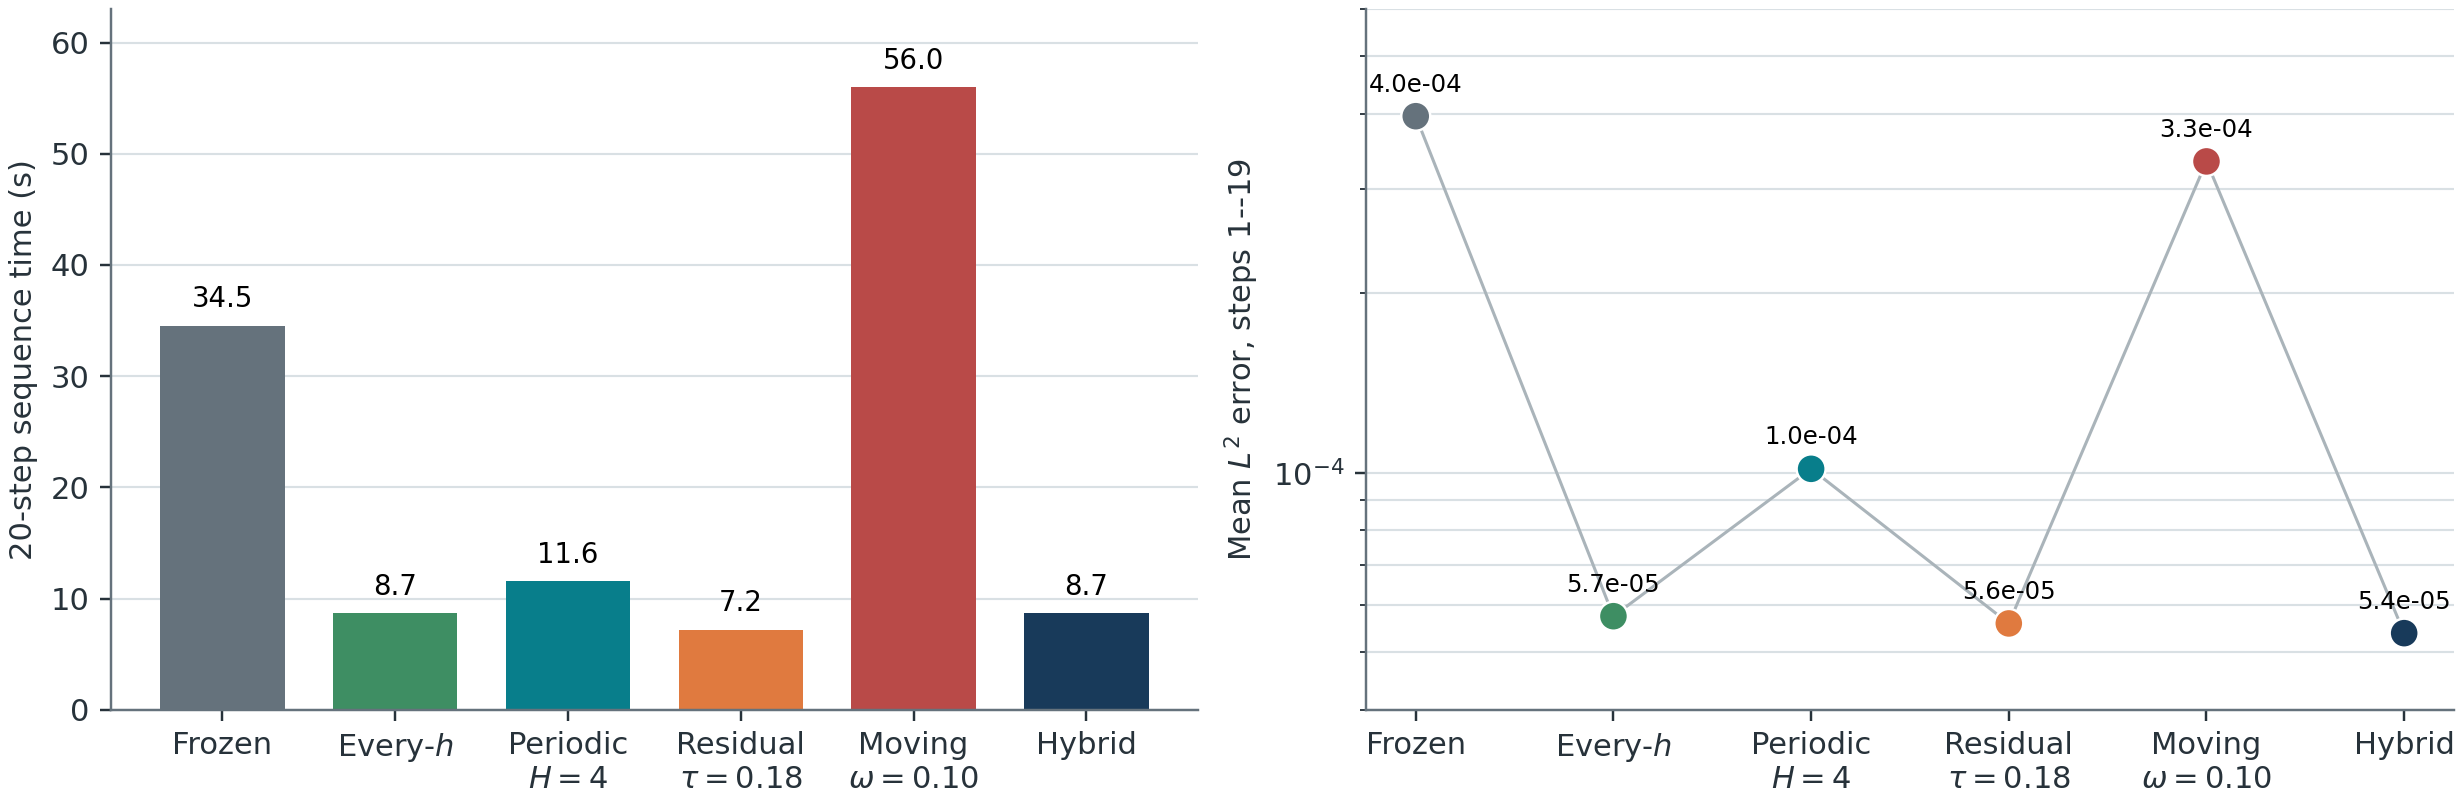
\includegraphics[width=0.98\textwidth]{mesh_policy_beamer_results.png}

  \vspace{-0.12cm}
  {\scriptsize
  Sequence time excludes the common initial setup; mean error is over steps
  $1$--$19$. Periodic: $H=4$; residual/hybrid: $\tau=0.18$,
  maximum reuse $=4$; moving/hybrid: $\omega=0.10$.}

  \vspace{0.08cm}
  \begin{beamercolorbox}[rounded=true,sep=0.25em,wd=0.96\textwidth]{block body}
    \centering\footnotesize
    \texttt{RESIDUAL\_H}: $4.78\times$ faster and $7.10\times$ more accurate
    than \texttt{FROZEN} in this test.
  \end{beamercolorbox}
\end{frame}

% 8
\begin{frame}{Where does the 20-step sequence time go?}
  \centering
  \scriptsize
  \setlength{\tabcolsep}{3.2pt}
  \renewcommand{\arraystretch}{1.12}
  \begin{tabular}{lrrrrrrr}
    \toprule
    Policy & $T_{\rm mesh}$ & $T_{\rm tree}$ & $T_{\rho}$ &
    $T_{\rm mom}$ & $T_{\rm eval}$ & $T_{\rm ctrl}$ & $T_{\rm seq}$\\
    \midrule
    Frozen       & 0.000 & 0.000 & 0.432 & 2.245 & 30.059 & 1.812 & 34.548\\
    Every-$h$    & 1.884 & 0.717 & 0.303 & 0.776 &  3.741 & 1.246 &  8.667\\
    Periodic $H=4$ & 0.507 & 0.220 & 0.310 & 1.332 &  8.093 & 1.113 & 11.576\\
    Residual     & 0.647 & 0.199 & 0.331 & 1.006 &  3.998 & 1.041 &  7.222\\
    Moving       & 7.774 & 5.782 & 3.855 & 1.729 & 29.909 & 6.912 & 55.961\\
    Hybrid       & 0.918 & 0.866 & 0.341 & 1.011 &  3.841 & 1.705 &  8.682\\
    \bottomrule
  \end{tabular}

  \vspace{0.18cm}
  \begin{columns}[T,onlytextwidth]
    \column{0.49\textwidth}
      \begin{block}{Construction and update costs}
        \scriptsize
        $T_{\rm mesh}$: $h/r$ mesh modification.\par
        $T_{\rm tree}$: hierarchy mapping and validation plus MAC
        neighbor/non-neighbor list construction.\par
        $T_{\rho}$: quadrature-cache construction after a rebuild, or source
        sampling on a reused mesh.
      \end{block}
    \column{0.49\textwidth}
      \begin{block}{Density-dependent calculation}
        \scriptsize
        $T_{\rm mom}$: leaf Cartesian moments and parent aggregation.\par
        $T_{\rm eval}$: direct neighbor and singular target integration plus
        far-field multipoles, at one barycenter per active leaf; it also
        accumulates the $L^2$ error.\par
        $T_{\rm ctrl}$: density-change/residual indicators and other overhead.
      \end{block}
  \end{columns}

  \vspace{0.04cm}
  {\scriptsize\color{muted}All entries are cumulative seconds; the common initial setup
  (2.30--2.85 s) is excluded from $T_{\rm seq}$.}
\end{frame}

% 9
\begin{frame}{Parameter sensitivity: update interval and mesh motion}
  \begin{columns}[T,onlytextwidth]
    \column{0.49\textwidth}
      \begin{block}{Periodic $h$-adaptation}
        \centering\footnotesize
        \begin{tabular}{rrrr}
          \toprule
          $H$ & updates & $T_{\rm seq}$ (s) & mean $E_{L^2}$\\
          \midrule
          2 & 9 & 9.54 & $7.14\times10^{-5}$\\
          4 & 4 & 11.58 & $1.02\times10^{-4}$\\
          8 & 2 & 17.66 & $1.82\times10^{-4}$\\
          \bottomrule
        \end{tabular}

        \vspace{0.18cm}
        \raggedright\scriptsize
        A larger $H$ postpones the first useful coarsening: more steps retain
        the initial $100\,656$-element mesh, so both time and error increase.
      \end{block}
    \column{0.49\textwidth}
      \begin{block}{Fixed-connectivity moving mesh}
        \centering\footnotesize
        \begin{tabular}{rrr}
          \toprule
          $\omega$ & $T_{\rm seq}$ (s) & mean $E_{L^2}$\\
          \midrule
          0.05 & 55.83 & $3.57\times10^{-4}$\\
          0.10 & 55.96 & $3.33\times10^{-4}$\\
          0.20 & 54.16 & $3.01\times10^{-4}$\\
          \bottomrule
        \end{tabular}

        \vspace{0.18cm}
        \raggedright\scriptsize
        Stronger motion improves tracking, but all variants retain $100\,656$
        elements and rebuild geometry-dependent lists at every step.
      \end{block}
  \end{columns}

  \vspace{0.10cm}
  \centering\footnotesize\color{navy}\bfseries
  Update timing changes both rebuild cost and subsequent evaluation cost.
\end{frame}

% 10
\begin{frame}[t]{Next step: let SCF evidence select the mesh policy}
  \centering\small
  \textbf{No update strategy is selected in advance.}
  Compare when to update, how to adapt, and what can be reused.

  \vspace{0.12cm}
  \begin{columns}[T,onlytextwidth]
    \column{0.32\textwidth}
      \begin{block}{Reuse baselines}
        \centering\footnotesize
        Frozen \; / \; periodic \; / \; every step
      \end{block}
    \column{0.32\textwidth}
      \begin{block}{Adaptive candidates}
        \centering\footnotesize
        Residual trigger \; / \; moving \; / \; hybrid
      \end{block}
    \column{0.32\textwidth}
      \begin{block}{Reusable structure}
        \centering\footnotesize
        Mesh \; / \; tree and MAC \; / \; quadrature
      \end{block}
  \end{columns}

  \vspace{0.10cm}
  \centering
  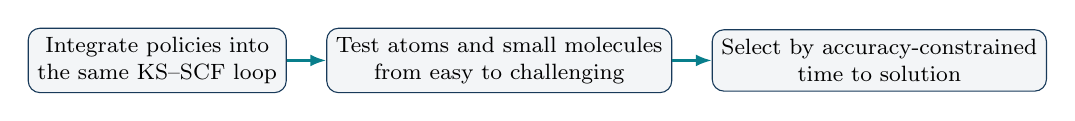
\begin{tikzpicture}[
      node distance=5mm,
      box/.style={draw=navy,rounded corners=1.5mm,fill=navy!5,
        minimum width=3.15cm,minimum height=0.78cm,align=center,font=\footnotesize},
      arr/.style={-{Latex[length=2mm]},thick,draw=teal}]
    \node[box] (scf) {Integrate policies into\\the same KS--SCF loop};
    \node[box,right=of scf] (test) {Test atoms and small molecules\\from easy to challenging};
    \node[box,right=of test] (select) {Select by accuracy-constrained\\time to solution};
    \draw[arr] (scf)--(test);
    \draw[arr] (test)--(select);
  \end{tikzpicture}

  \vspace{0.10cm}
  \begin{block}{Common decision criteria}
    \centering\scriptsize
    Total SCF time and iteration count \quad $\vert\Delta E\vert$ and density error
    \quad force accuracy \quad memory \quad robustness
  \end{block}

  \vspace{-0.02cm}
  \centering\footnotesize\bfseries\color{navy}
  The objective is not the cheapest step, but the fastest reliable SCF solution.
\end{frame}

\end{document}
